%!TEX TS-program = xelatex
%!TEX encoding = UTF-8 Unicode
%!TeX spellcheck = it_IT
%!TEX root = ../tesi.tex

\chapter{Simulazioni}\label{chap:simulazioni}
% INTRO: cosa c'è in questa sezione?
Dopo aver illustrato il protocollo in esame e il modello di propagazione utilizzato, si passa ora alla fase di valutazione.
Il capitolo procederà, quindi, nel dettaglio delle diverse simulazioni effettuate analizzando i relativi risultati.
% Ogni capitolo presenterà un gruppo di simulazioni, che differiscono dagli altri per scenario applicativo e configurazione.
% NB: non è bellissimo
%
\section{Configurazione a griglia}\label{sec:configurazione-griglia}
% \subsection{Panoramica}
% Simulazioni codice barichello:
%  - struttura simulazioni
%  - grafici
%  - risulati
Il primo gruppo di simulazioni ha lo scopo di analizzare il comportamento del protocollo Fast Broadcast con e senza edifici all'interno
di un ambiente conosciuto;
per questo motivo, la configurazione è la stessa presentata nel documento originale \cite{Barichello2017propagazione}, a cui sono stati aggiunti gli edifici.
Lo scenario è una città fittizia con strade a griglia in stile Manhattan di lunghezza $4000$ metri e distanti l'una dall'altra $300$ metri.
I veicoli sono disposti a $12$ metri di distanza per un totale di $8064$.
Il veicolo dal quale ha inizio la fase di inoltro (generazione del primo messaggio di inoltro) è posizionato
al centro della griglia, in modo da avere una propagazione teoricamente uniforme;
per facilità verrà chiamato veicolo \textit{zero}.
Seguendo l'idea originale, è stata definita anche un circonferenza di raggio pari a $1000\pm12$ metri, utilizzata per definire alcune metriche che verranno descritte in seguito;
la circonferenza ha centro in corrispondenza del veicolo zero.
Il raggio trasmissivo effettivo assume due valori possibili: $300$ metri o $500$ metri;
il tutto è riassunto in Tabella~\ref{tab:parametri-simulazioni-barichello}.

Per valutare il protocollo sono stati presi in esame diversi parametri: la copertura totale e la copertura sulla circonferenza,
il numero di salti necessari per raggiungere il bordo della griglia, il numero totale di messaggi di inoltro ricevuti e inviati.
In modo da aver un metro di paragone per il protocollo Fast Broadcast, quest'ultimo è stato comparato con altri due metodi, chiamati \statica e \staticb,
che utilizzano una stima fissa del raggio tramissivo, rispettivamente di $300$ e $500$ metri.

Gli edifici sono stati creati apposititamente, in modo che ogni edificio fosse contenuto all'interno dello spazio creato dalle strade.
Così facendo, risultano $169$ edifici di $295$x$295$ metri (i muri sono distanziati di $5$ metri dalla strada).
%
\begin{table}[htbp]
	\centering
	\begin{tabular}{| L{.4\linewidth} | r  l |}
		\toprule
		Parametro															&			Valore 				&					\\
		\thickerline
		Lunghezza delle strade								&			$4000$				& m				\\
		Distanza fra le strade								&			$300$					& m				\\
		Distanza fra i veicoloi								&			$12$ 					& m				\\
		Circonferenza													&			$1000\pm12$		& m				\\
		Posizione del veicolo zero						&			centrale			&					\\
		Numero di simulazioni									&			$50$					&					\\
		\thickerline
		Dimensioni pacchetto				&				$164$							&			byte		\\	\hline
		Standard tramissione				&				$802.11$b					&							\\	\hline
		Frequenza										&				$2.4$							&			GHz			\\	\hline
		Banda del canale						&				$22$							&			MHz			\\	\hline
		Velocità di tramissione			&				$11$							&			Mbps		\\	\hline
		Potenza trasmissione				&				$4,6$-$13,4$			&			dBm			\\	\hline
		Raggio tramissivo						&				$300$-$500$				&			m				\\	\hline
		Codifica										&				DSSS\footnotemark	&							\\	\hline
		Modello di propagazione			&				Two-Ray Ground		&							\\	\hline
		Modello di ombreggiatura		&				A ostacoli				&							\\
		\bottomrule
	\end{tabular}
	\caption{Configurazione dei parametri per le simulazioni.\label{tab:parametri-simulazioni-barichello}}
\end{table}
\footnotetext{\textit{Direct Sequence Spread Spectrum}}	% TODO controllare la posizone, che sia nella stessa pagina della tabella.
%
% \begin{figure}[htbp]
% 	\centering
% 	\begin{center}
% 		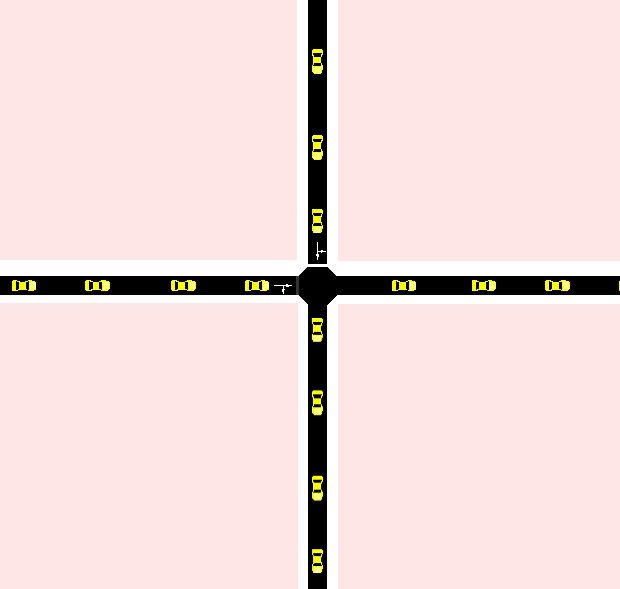
\includegraphics[width=.4\textwidth]{griglia-dettaglio-2.png}
% 	\end{center}
% 	\label{fig:griglia-dettaglio}\caption{Dettaglio della configurazione a griglia: in nero le strade e in giallo gli edifici.}
% \end{figure}
%
\subsection{Risultati}\label{sec:configurazione-griglia-risultati}
%
% TODO
%
\section{Scenario urbano reale} % un titolo migliore no?
Le configurazioni precedenti avevano il difetto di essere poco veritiere, sia dal punto di vista della topologia stradale
che sulla geometria degli edifici.
In questo gruppo di simulazioni, invece, si è voluto valutare Fast Broadcast all'interno di uno scenario quanto più reale possibile.
Sono state scelte due città, Padova (IT) e Los Angeles (California, USA) (Figura~\ref{fig:scenari-la-pd-osm}), definite due aree nella zona centrale di circa $5$ kilometri quadrati (Figura~\ref{fig:scenari-la-pd-osm})
e, seguendo il procedimento descritto nella Sezione~\ref{sec:sumo}, si sono estratte le informazioni necessarie alla simulazione.
Altre informazioni sulla configurazione sono elencati in Tabella~\ref{tab:parametri-simulazioni-pd-la}.

La scelta è ricaduta su Los Angeles poiché la sua rete stradale è molto simile a una griglia in stile Manhattan, come anche nello scenario precedente,
mentre Padova (sede anche dell'Università dove si è svolto questo lavoro) ha una toplogià più irregolare, con strade più strette ed edifici a ridosso di queste,
zone pedonali e ZTL.
%
\begin{table}[htbp]
	\centering
	  \begin{tabular}{| L{.35\linewidth} | C{.01\linewidth} | C{.04\linewidth} | L{.15\linewidth} | L{.15\linewidth} |}
			\toprule
			\multicolumn{3}{|m{.3\linewidth}|}{\multirow{2}{*}{}}														&		\multicolumn{2}{c|}{Scenario}						\\ \cline{4-5}
			\multicolumn{3}{|m{.3\linewidth}|}{}																						&		Padova				&			Los Angeles					\\
			\thickerline
			\multicolumn{2}{|m{.25\linewidth}|}{\multirow{2}{*}{Latitudine}}				&		N	 	& 	$45,4171$				&			$33,9654$					\\ \cline{3-5}
			\multicolumn{2}{|m{.25\linewidth}|}{}																		&		S	 	& 	$45,3981$				&			$33,9478$					\\ \hline
			\multicolumn{2}{|l|}{\multirow{2}{*}{Longitudine}}											&		O	 	& 	$11,8654$				&			-$118,3260$				\\ \cline{3-5}
			\multicolumn{2}{|l|}{}																									&		E	 	& 	$11,8923$				&			-$118,3055$				\\ \hline
			\multicolumn{3}{|l|}{Area approssimativa [km$^2$]}															&		\multicolumn{2}{c|}{$5$}								\\ \hline
			\multicolumn{3}{|l|}{Distanza fra veicoli [metri]}															&		\multicolumn{2}{c|}{$25$}								\\ \hline
			\multicolumn{3}{|l|}{Numero di veicoli}																					&		$2224$					&					$1905$				\\ \hline
			\multicolumn{3}{|l|}{Numero di edifici}																					&		$6322$					&					$8241$				\\ \hline
			\multicolumn{3}{|l|}{Circonferenza [metri]}																			&		\multicolumn{2}{c|}{$1000\pm25$}				\\ \hline
			\multicolumn{3}{|l|}{Posizione del veicolo zero}																&		\multicolumn{2}{c|}{centrale}						\\ \hline
			\multicolumn{3}{|l|}{Numero di simulazioni}																			&		\multicolumn{2}{c|}{$50$}								\\
			\bottomrule
	  \end{tabular}
	\caption{Parametri della topologia per gli scenari urbani.\label{tab:parametri-simulazioni-pd-la}}
\end{table}
%
\begin{figure}[htbp]
	\centering
		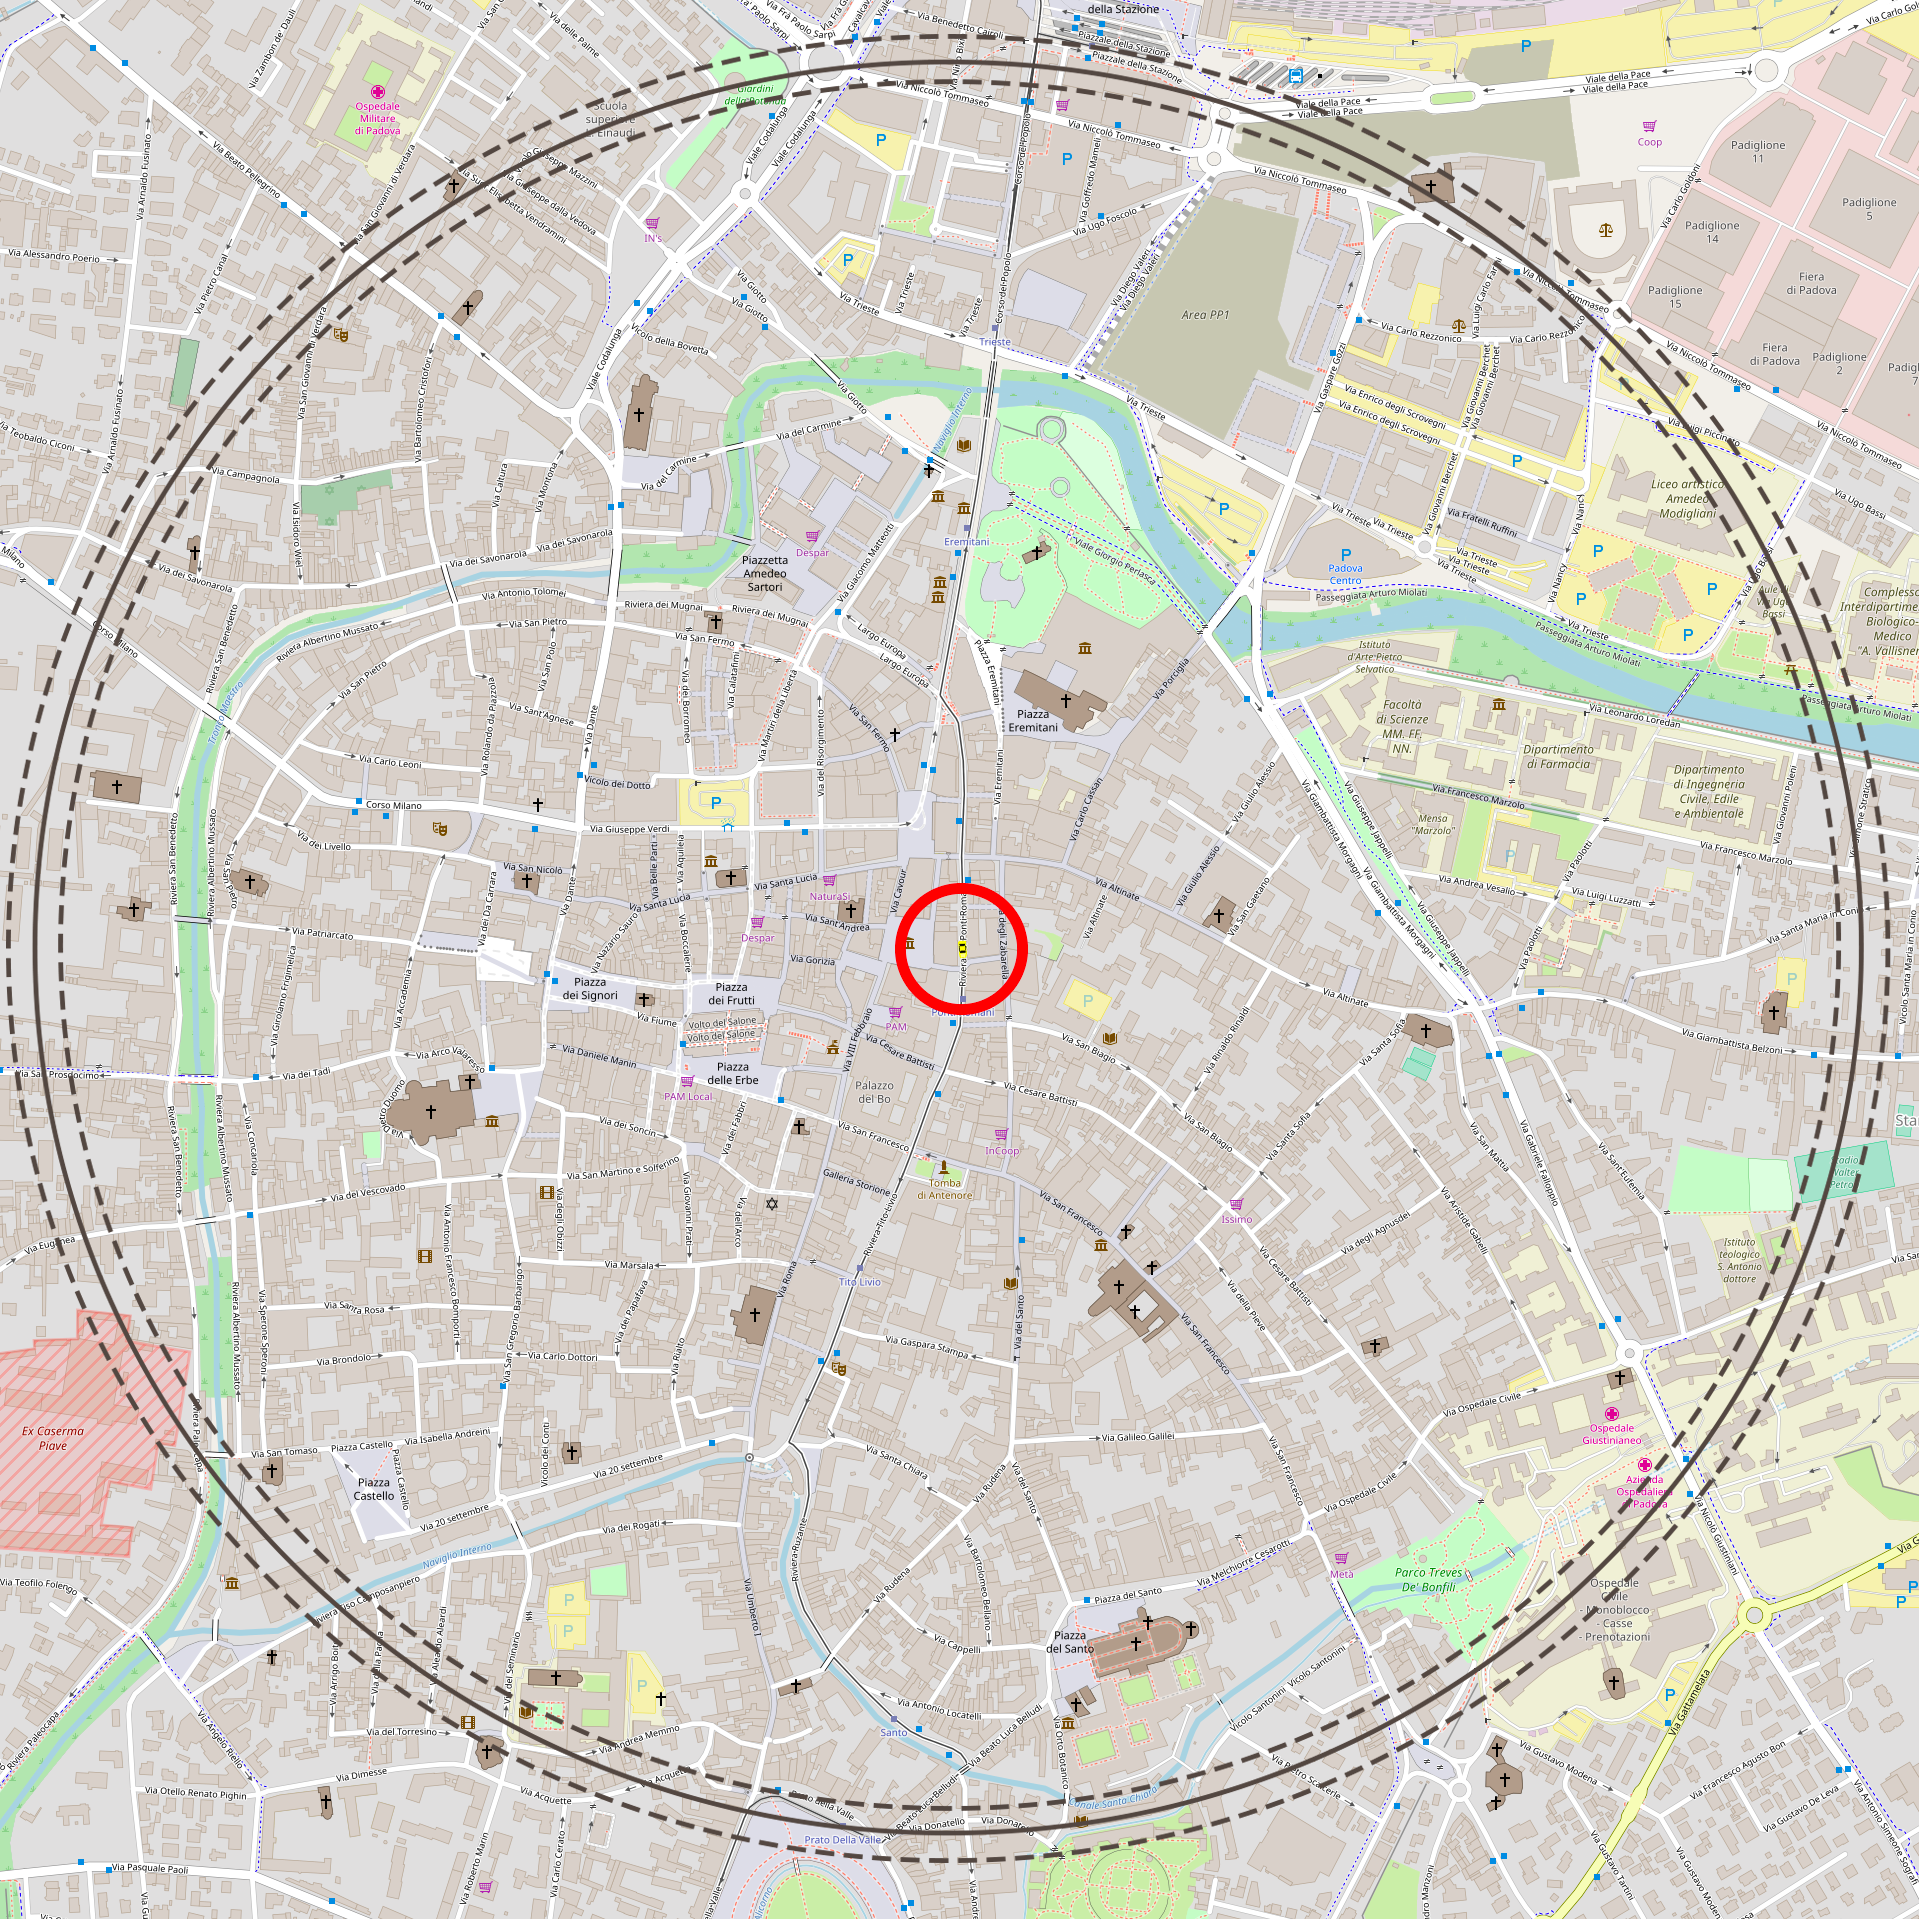
\includegraphics[width=.49\textwidth]{osm_web-pd-2x2.png}
		\hfill
		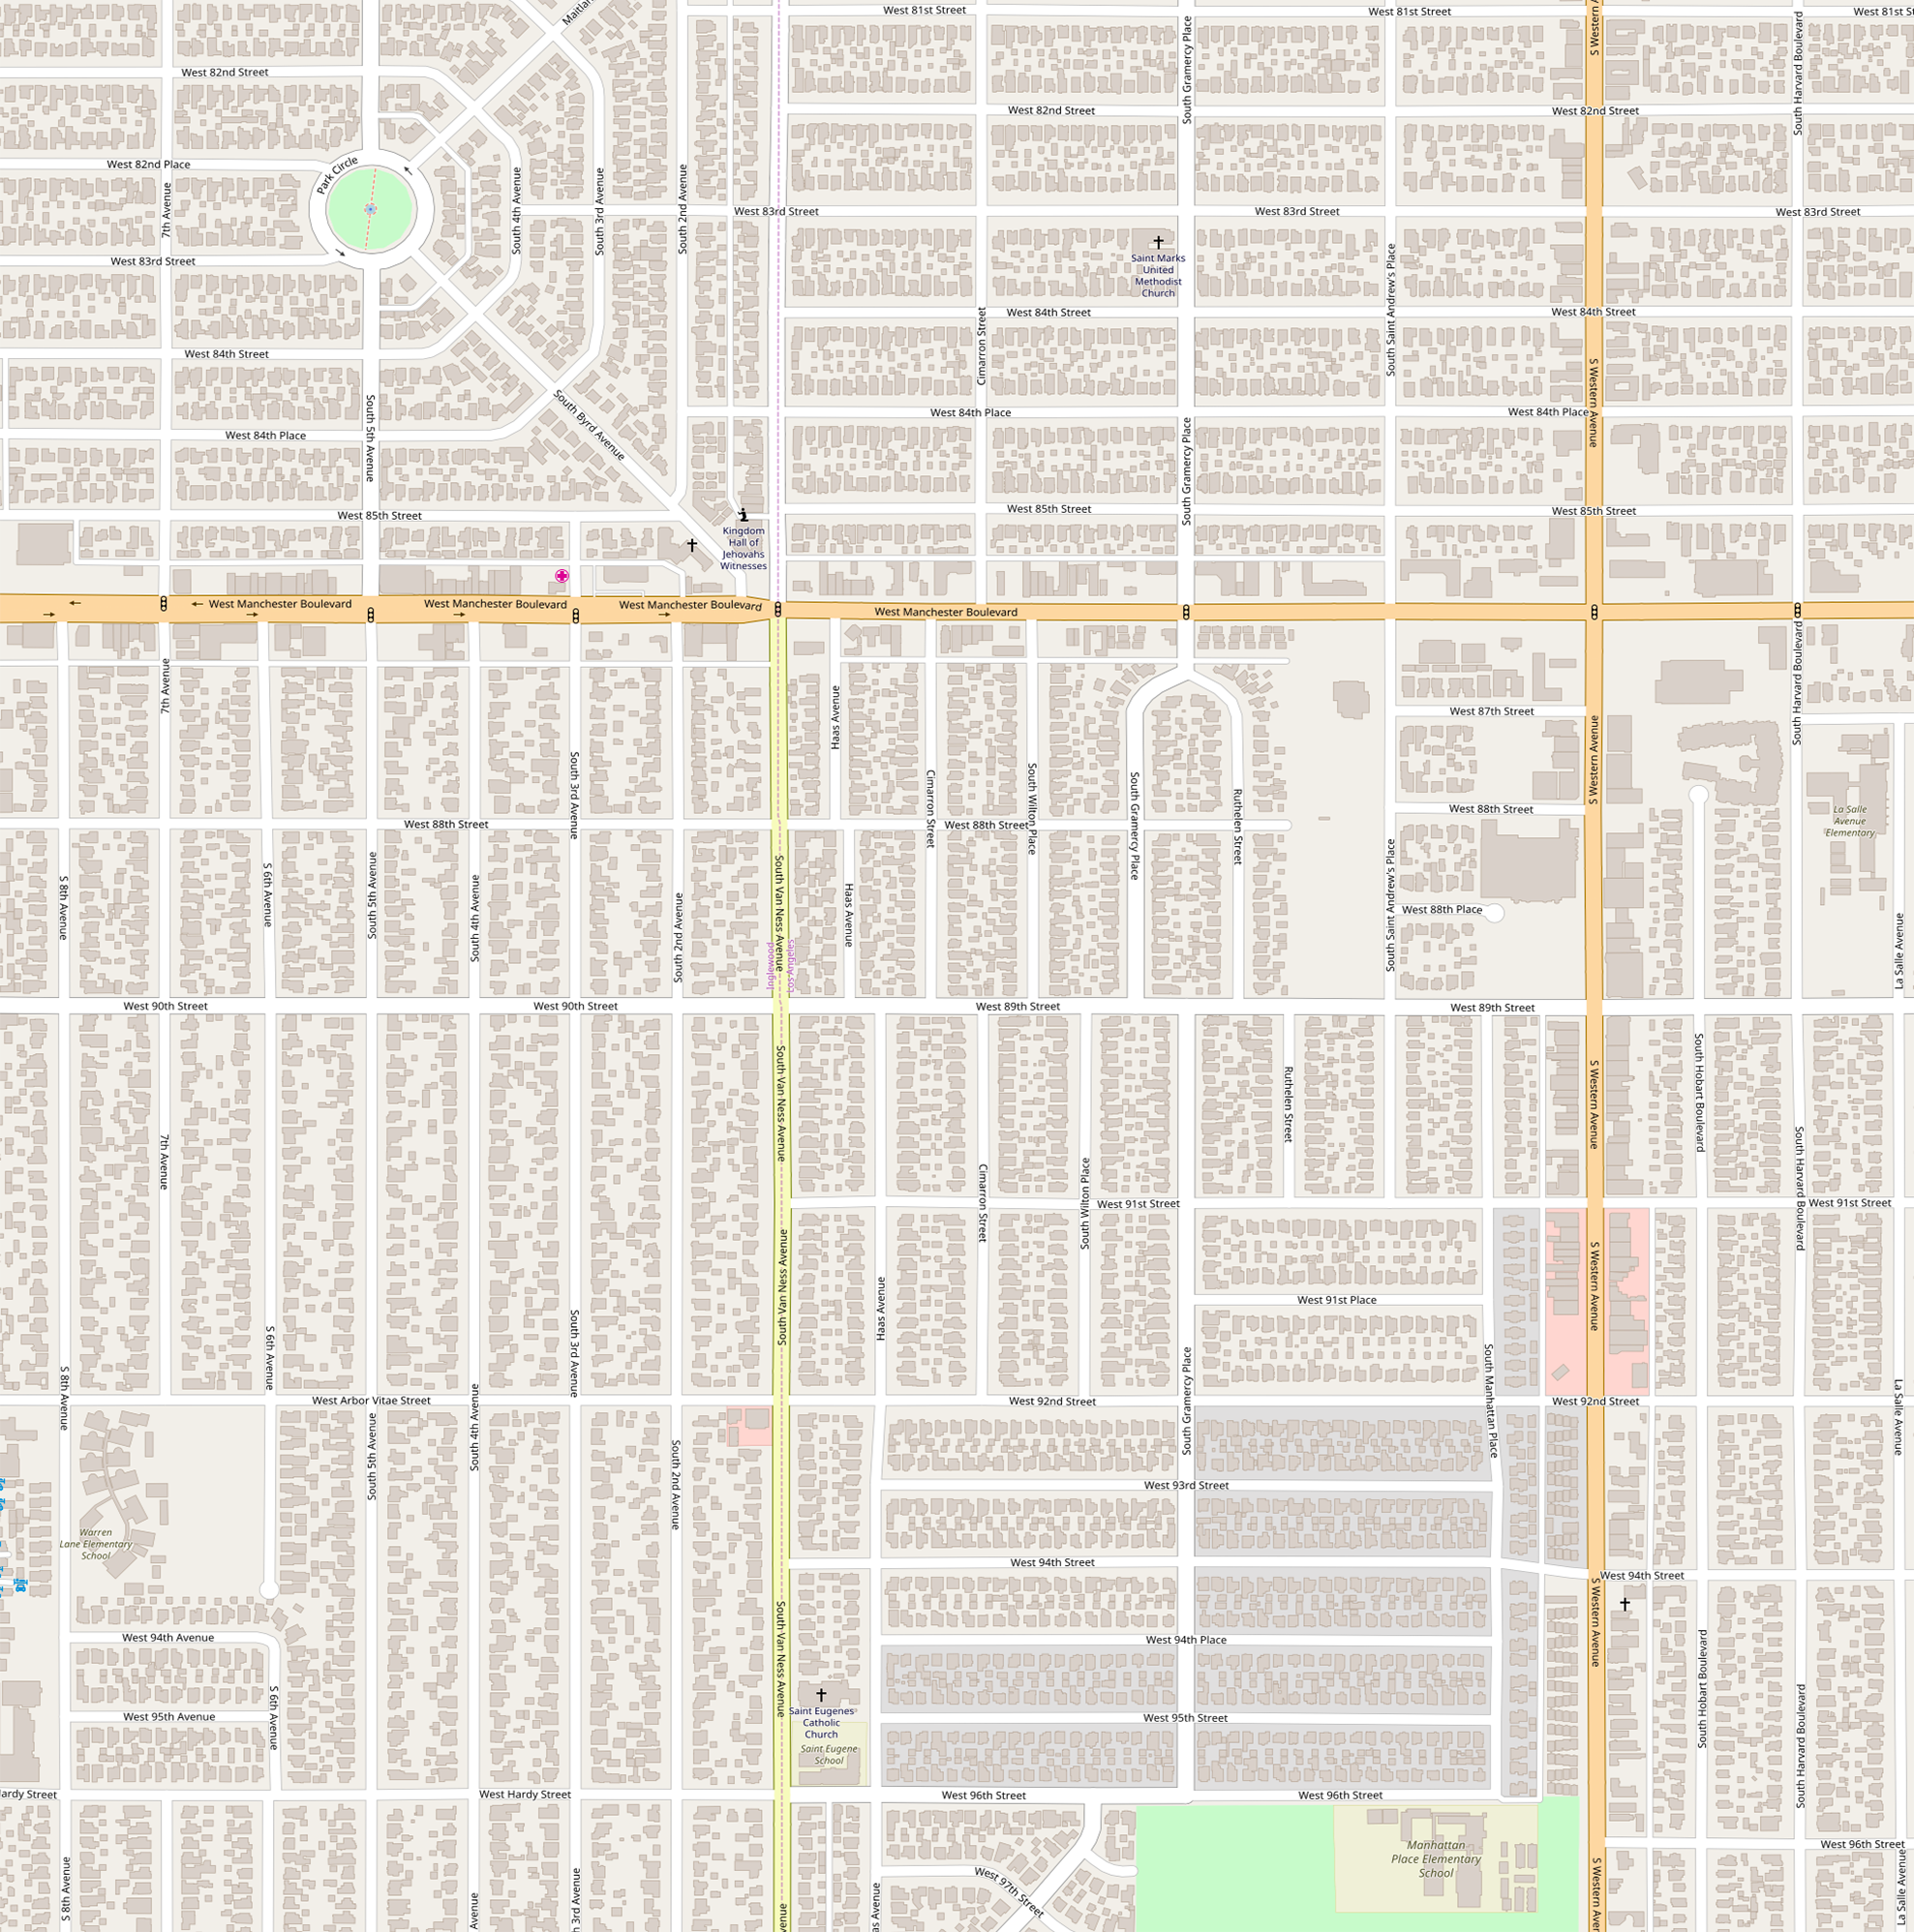
\includegraphics[width=.49\textwidth]{osm_web-la-2x2.png}
\caption{Una vista delle aree selezionate per le simulazioni; a sinistra la città di Padova e a destra Los Angeles (fonte: OSM).
Il cerchio rosso evidenzia la posizione del nodo di partenza mentre i tre rimanenti rappresentano il perimetro della circonferenza
e i due intervalli di confidenza.\label{fig:scenari-la-pd-osm}}
\end{figure}
%
Anche in questo gruppo di simulazioni sono state utilizzate le medesime metriche del caso precendente,
fatta eccezione per il numero di salti che ora sono per raggiungere la circonferenza, non il bordo dello scenario.
Questo perché nella configurazione a griglia lungo il perimetro esterno erano sicuramente posizionati dei veicoli,
mentre ora il limite ``quadratico'' dell'area è ideale (non tutte le strade finisco esattamente sul bordo della mappa).
%
\subsection{Los Angeles}\label{subsec:risultati-la}
%
\subsection{Padova}\label{subsec:risultati-pd}

% \begin{figure}[htbp]
% 	\centering
% 		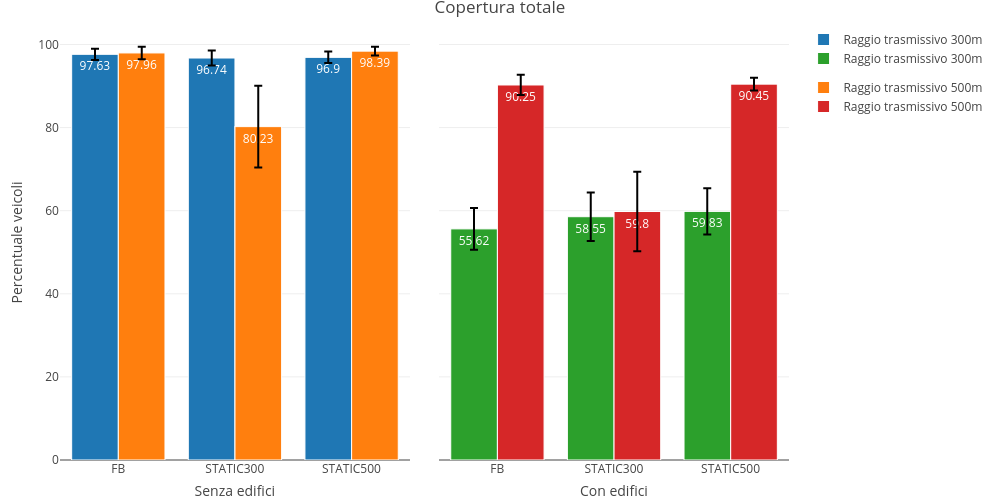
\includegraphics[width=\textwidth]{grafici/pd_copertura_totale.png}
% 		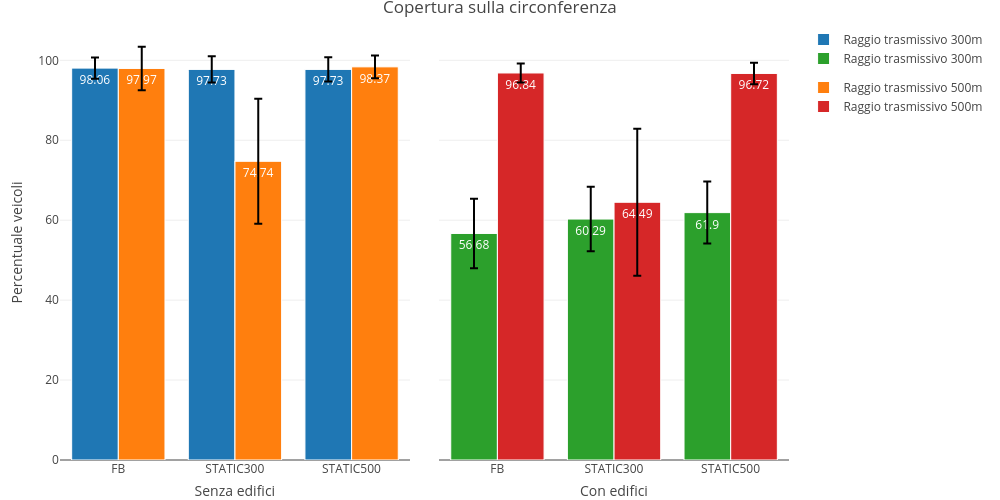
\includegraphics[width=\textwidth]{grafici/pd_copertura_circonferenza.png}
% \caption{Copertura dei veicoli totale e sulla circonferenza dei veicoli\label{fig:risultati-padova-copertura}}
% \end{figure}
% %
% \begin{figure}[htbp]
% 	\centering
% 		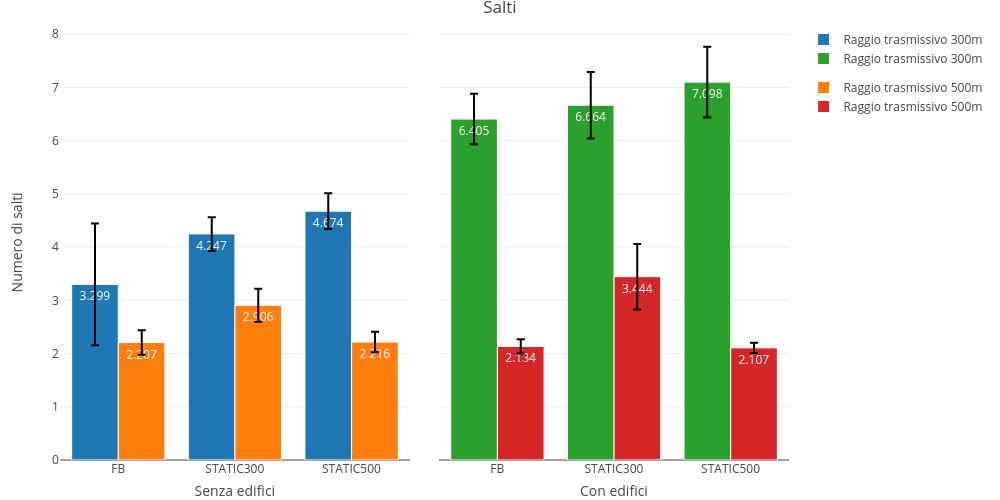
\includegraphics[width=\textwidth]{grafici/pd_salti.png}
% \caption{Numero di salti necessario per raggiungere la circonferenza dei veicoli\label{fig:risultati-padova-salti}}
% \end{figure}
% %
% \begin{figure}[htbp]
% 	\centering
% 		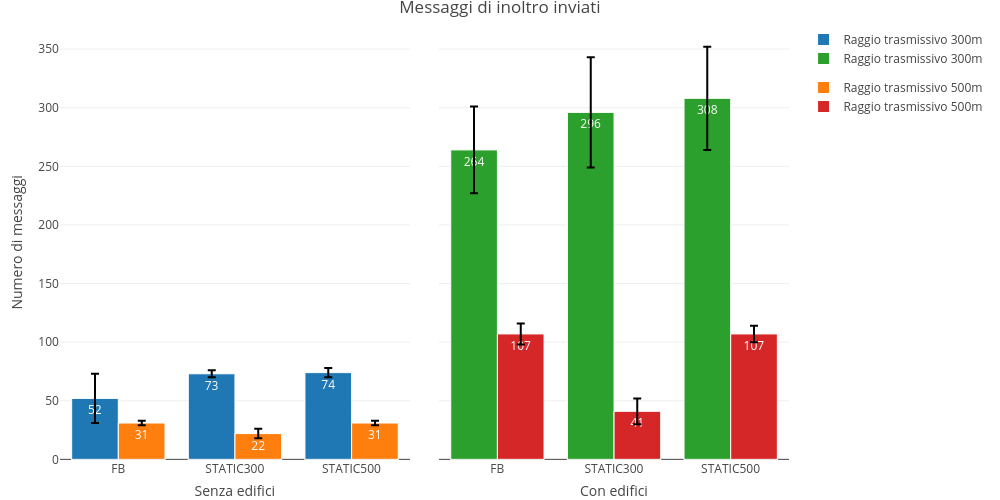
\includegraphics[width=\textwidth]{grafici/pd_messaggi_inviati.png}
% 		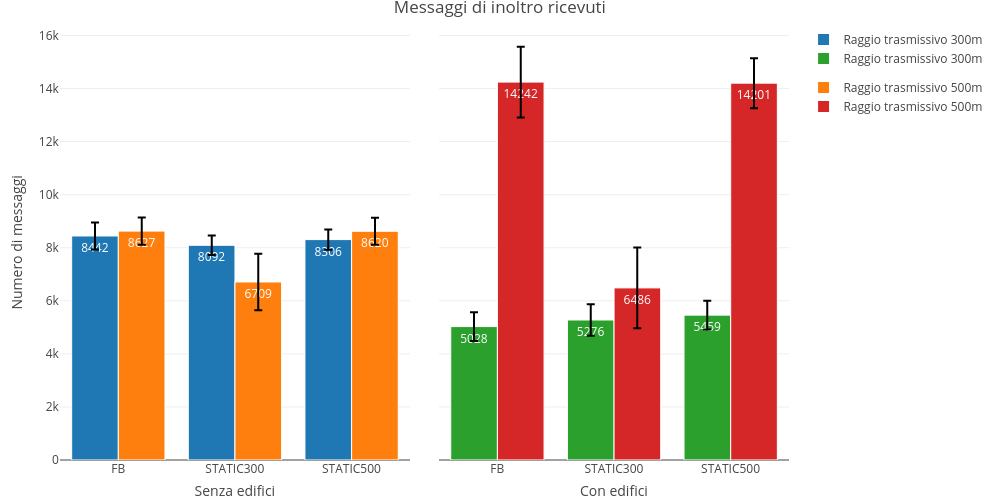
\includegraphics[width=\textwidth]{grafici/pd_messaggi_ricevuti.png}
% \caption{Quantità di messaggi di inoltro durante la simulazione.\label{fig:risultati-padova-messaggi}}
% \end{figure}
